\documentclass[a4paper,12pt,oneside]{book}

%-------------------------------Start of the Preable------------------------------------------------
\usepackage[english]{babel}
\usepackage{blindtext}
%packagr for hyperlinks
\usepackage{hyperref}
\hypersetup{
    colorlinks=true,
    linkcolor=blue,
    filecolor=magenta,      
    urlcolor=cyan,
}

\urlstyle{same}
%use of package fancy header
\usepackage{fancyhdr}
\setlength\headheight{26pt}
\fancyhf{}
%\rhead{
\includegraphics[width=1cm]{logo}}
\lhead{\rightmark}
\rhead{
\includegraphics[width=1cm]{logo}}
\fancyfoot[RE, RO]{\thepage}
\fancyfoot[CE, CO]{\href{http://www.e-yantra.org}{www.e-yantra.org}}

\pagestyle{fancy}

%use of package for section title formatting
\usepackage{titlesec}
\titleformat{\chapter}
  {\Large\bfseries} % format
  {}                % label
  {0pt}             % sep
  {\huge}           % before-code
 
%use of package tcolorbox for colorful textbox
\usepackage[most]{tcolorbox}
\tcbset{colback=cyan!5!white,colframe=cyan!75!black,halign title = flush center}

\newtcolorbox{mybox}[1]{colback=cyan!5!white,
colframe=cyan!75!black,fonttitle=\bfseries,
title=\textbf{\Large{#1}}}

%use of package marginnote for notes in margin
\usepackage{marginnote}

%use of packgage watermark for pages
%\usepackage{draftwatermark}
%\SetWatermarkText{
\includegraphics{logo}}
\usepackage[scale=2,opacity=0.1,angle=0]{background}
\backgroundsetup{
contents={
\includegraphics{logo}}
}

%use of newcommand for keywords color
\usepackage{xcolor}
\newcommand{\keyword}[1]{\textcolor{red}{\textbf{#1}}}

%package for inserting pictures
\usepackage{graphicx}

%package for highlighting
\usepackage{color,soul}

%new command for table
\newcommand{\head}[1]{\textnormal{\textbf{#1}}}


%----------------------End of the Preamble---------------------------------------


\begin{document}

%---------------------Title Page------------------------------------------------
\begin{titlepage}
\raggedright
{\Large eYSIP 2017\\[1cm]}
{\Huge\scshape Modeling, Designing and Simulation of Grow Box \\[.1in]}
\vfill
\begin{flushright}
{\large Intern Abhishek Kumar Verma \\}
{\large Mentors \hspace{35pt} Lohit Penubaku \\}
{\large Vishwanathan Iyer \\}
{\large Ajit Harpude \\}
{\large Rucmenya Bessariya \\}
{\large Duration of Internship: $ 22/05/2017-07/07/2017 $ \\}
\end{flushright}

{\itshape 2017, e-Yantra Publication}
\end{titlepage}
%-------------------------------------------------------------------------------

\chapter[Project Tag]{Modeling, Designing and Simulation of Grow Box}
\section*{Abstract}
Grow Box is partially or completely closed system to grow plants.So, in order to grow plant, environment needs to be provided. The existing Grow Box has all the necessary properties and has potential to be a product. It's now time to put everything in order, in terms of hardware, a good water container, flexibility and its structure. By doing this not only it will make market appealing, but also brings in an design attitude towards project development cycle. This report contains process to design the Grow Box Hardware along with flow simulation of air inside the system. It also contains the step by step process to assemble the Grow Box.

\subsection*{Completion status}
Two version of Grow Box has been designed. Version2 has been fabricated with all the Electronics hardware.

\section{Modeling and Designing}
Design consideration
\begin{itemize}
\item Air Circulation
\item Temperature Control
\item Light Positioning
\item Size
\item Modularity
\item Cost
\item DIY Design
\item Aesthetics
\end{itemize}

\subsection{Grow Box V0}
This is first prototype to be fabricated.\\
\includegraphics[width=200pt]{growboxversio0}\\
\href{https://www.youtube.com/watch?v=nuCj2OUl2X8}{Air Flow Simulation in Grow Box Version0} in Solid Works\\
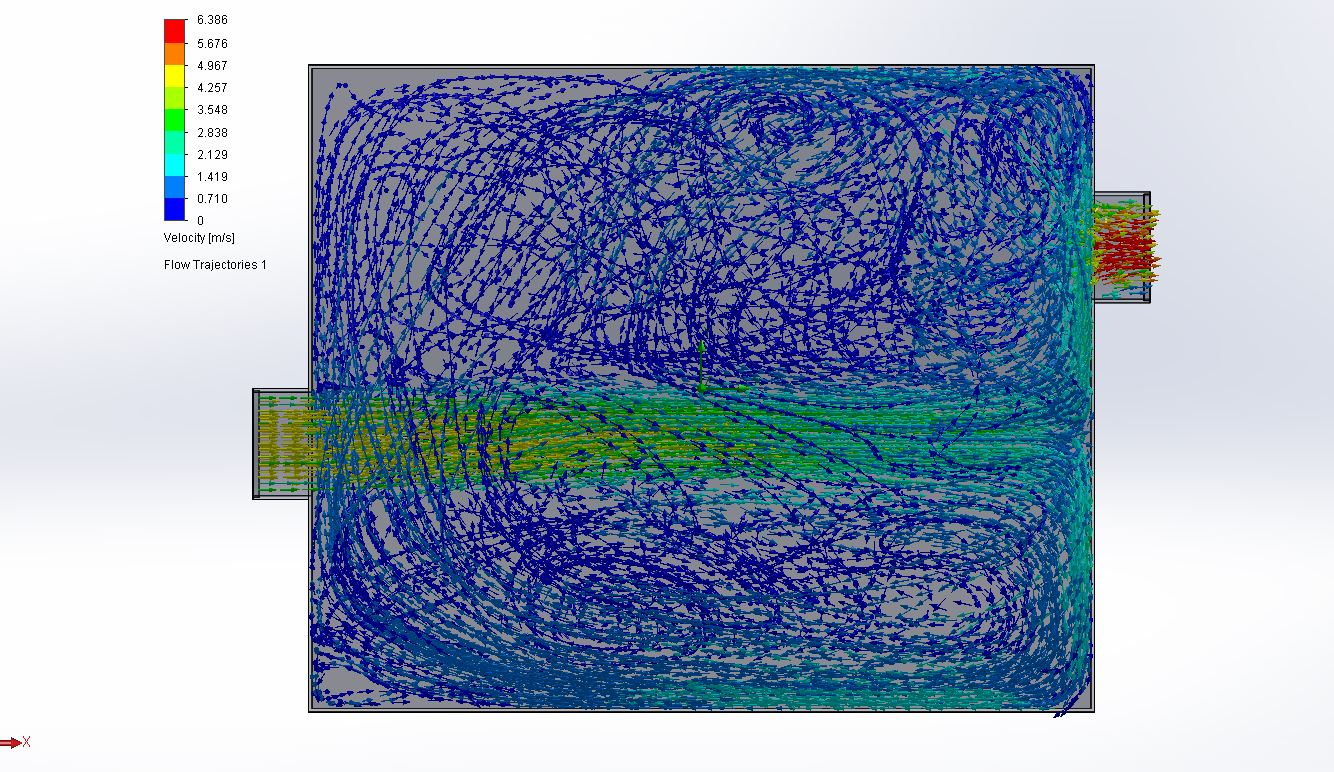
\includegraphics[width=200pt]{version_0_FV}
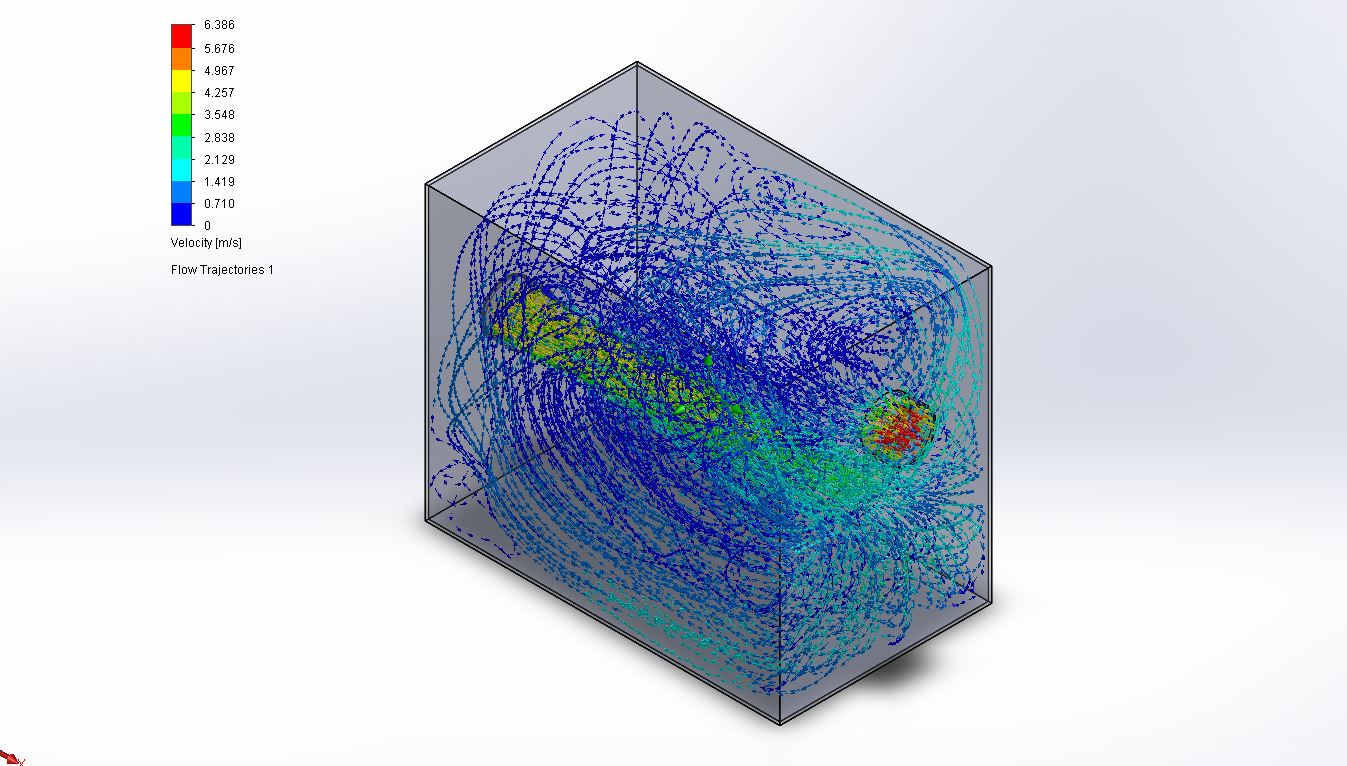
\includegraphics[width=200pt]{version_0_ISO}

\subsection{Grow Box V1}
This is the \href{https://www.youtube.com/watch?v=sGrjrwHcsWk}{first version} and is designed in Autodesk Fusion 360.\\
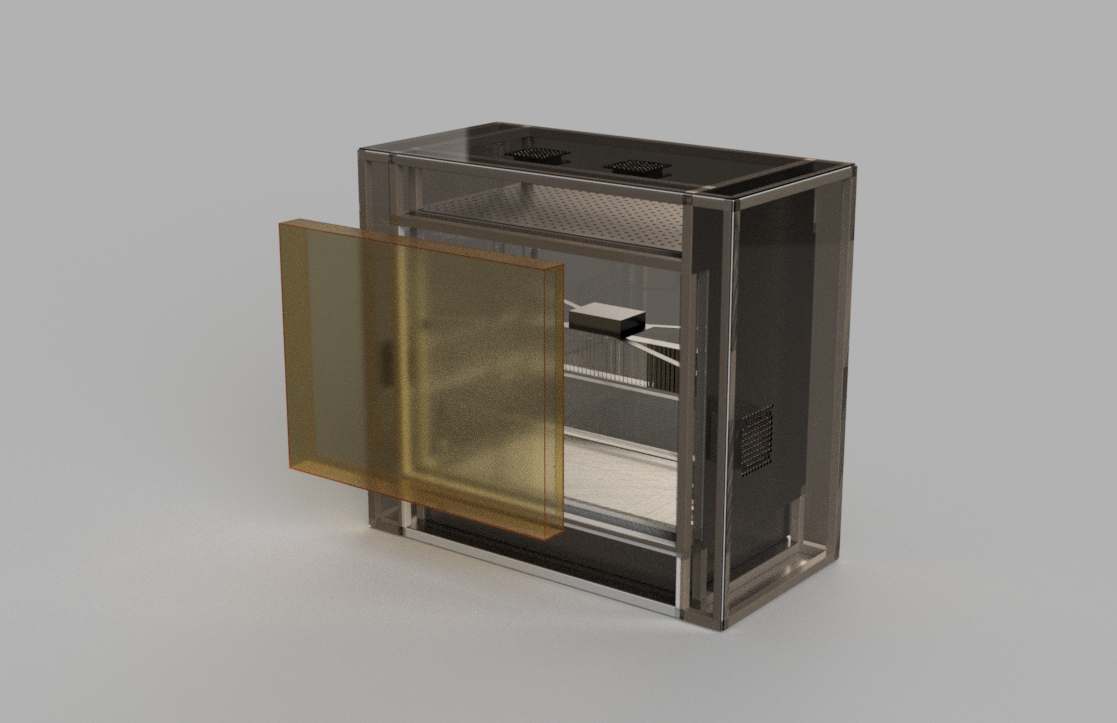
\includegraphics[width=200pt]{version_1}\\
To see the 3D Model  \href{http://a360.co/2rCJyYc}{Click}\\
\href{https://www.youtube.com/watch?v=ab_HcFKEwkE}{Air Flow Simulation in Grow Box Version1} in Solid Works\\
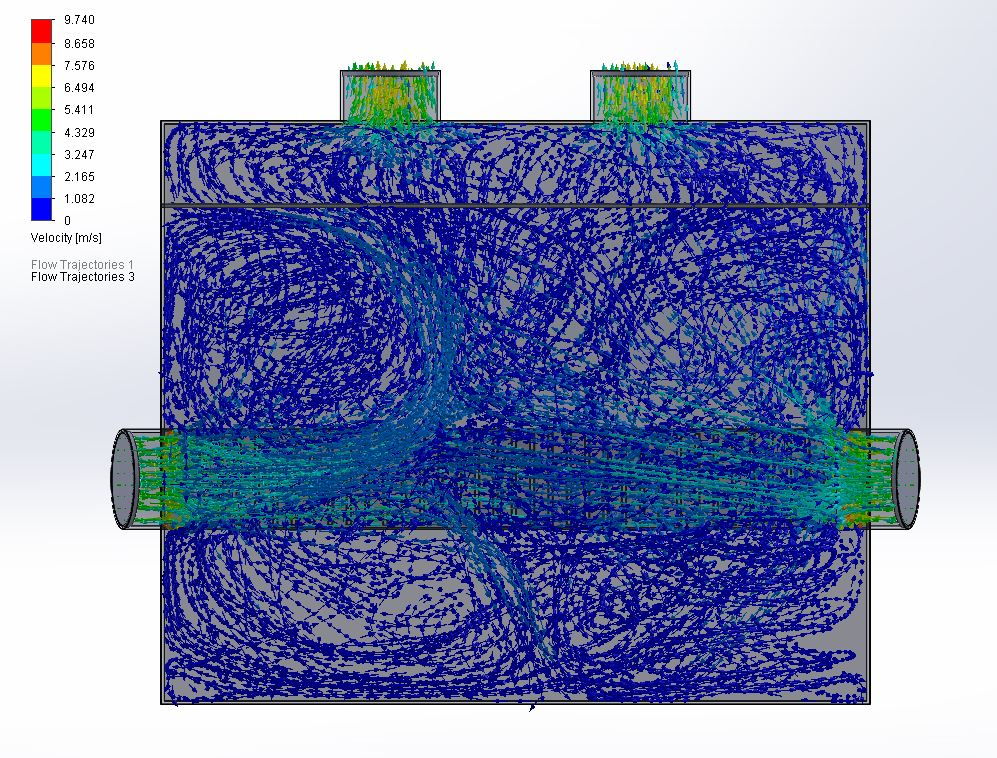
\includegraphics[width=200pt]{version_1_FV}
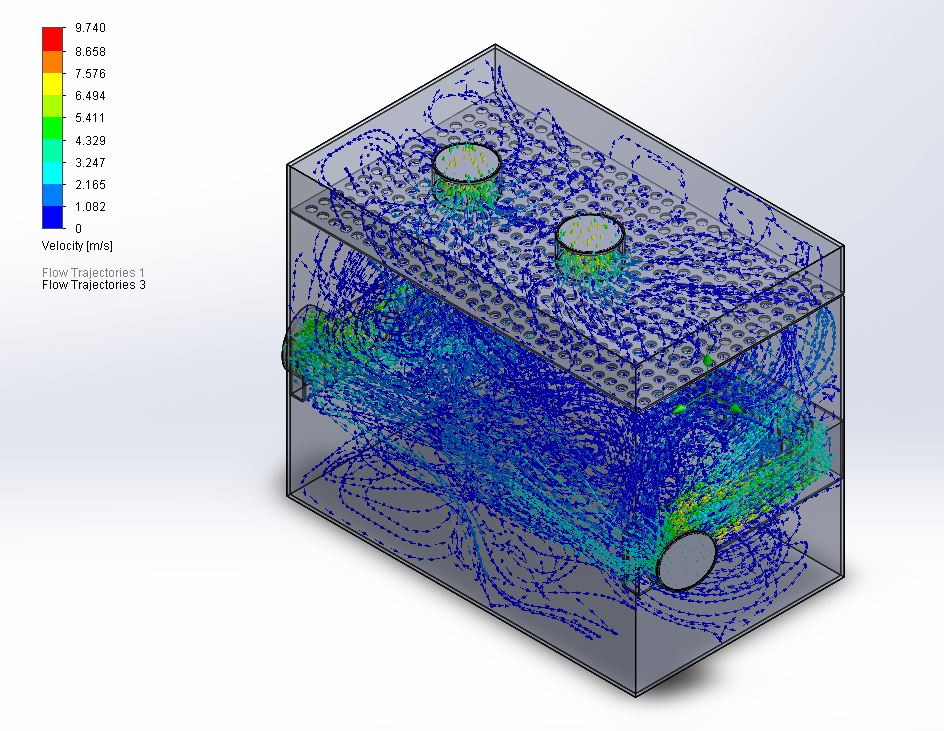
\includegraphics[width=200pt]{version_1_ISO}\\
Advantages of version1 are as follows:-
\begin{itemize}
    \item Good air flow inside the Grow Box.
    \item This design is modular. So, it can be stacked vertically or horizontally by just changing the Aluminum Tube with MS Tubes.
    \item Water storage facility is present.
    \item Light position can be changed as required
    \item DIY Design.
\end{itemize}
The disadvantage of this model are as follows- 
\begin{itemize}
\item The cost of fabrication of this model is high due to complex design. 
\item This design is bigger in size compared to existing model.
\end{itemize}

\subsection{Grow Box V2}
This is the \href{https://www.youtube.com/watch?v=TTjnuqw7IV8}{Second version} and is designed in Autodesk Fusion 360. This model has been fabricated.\\
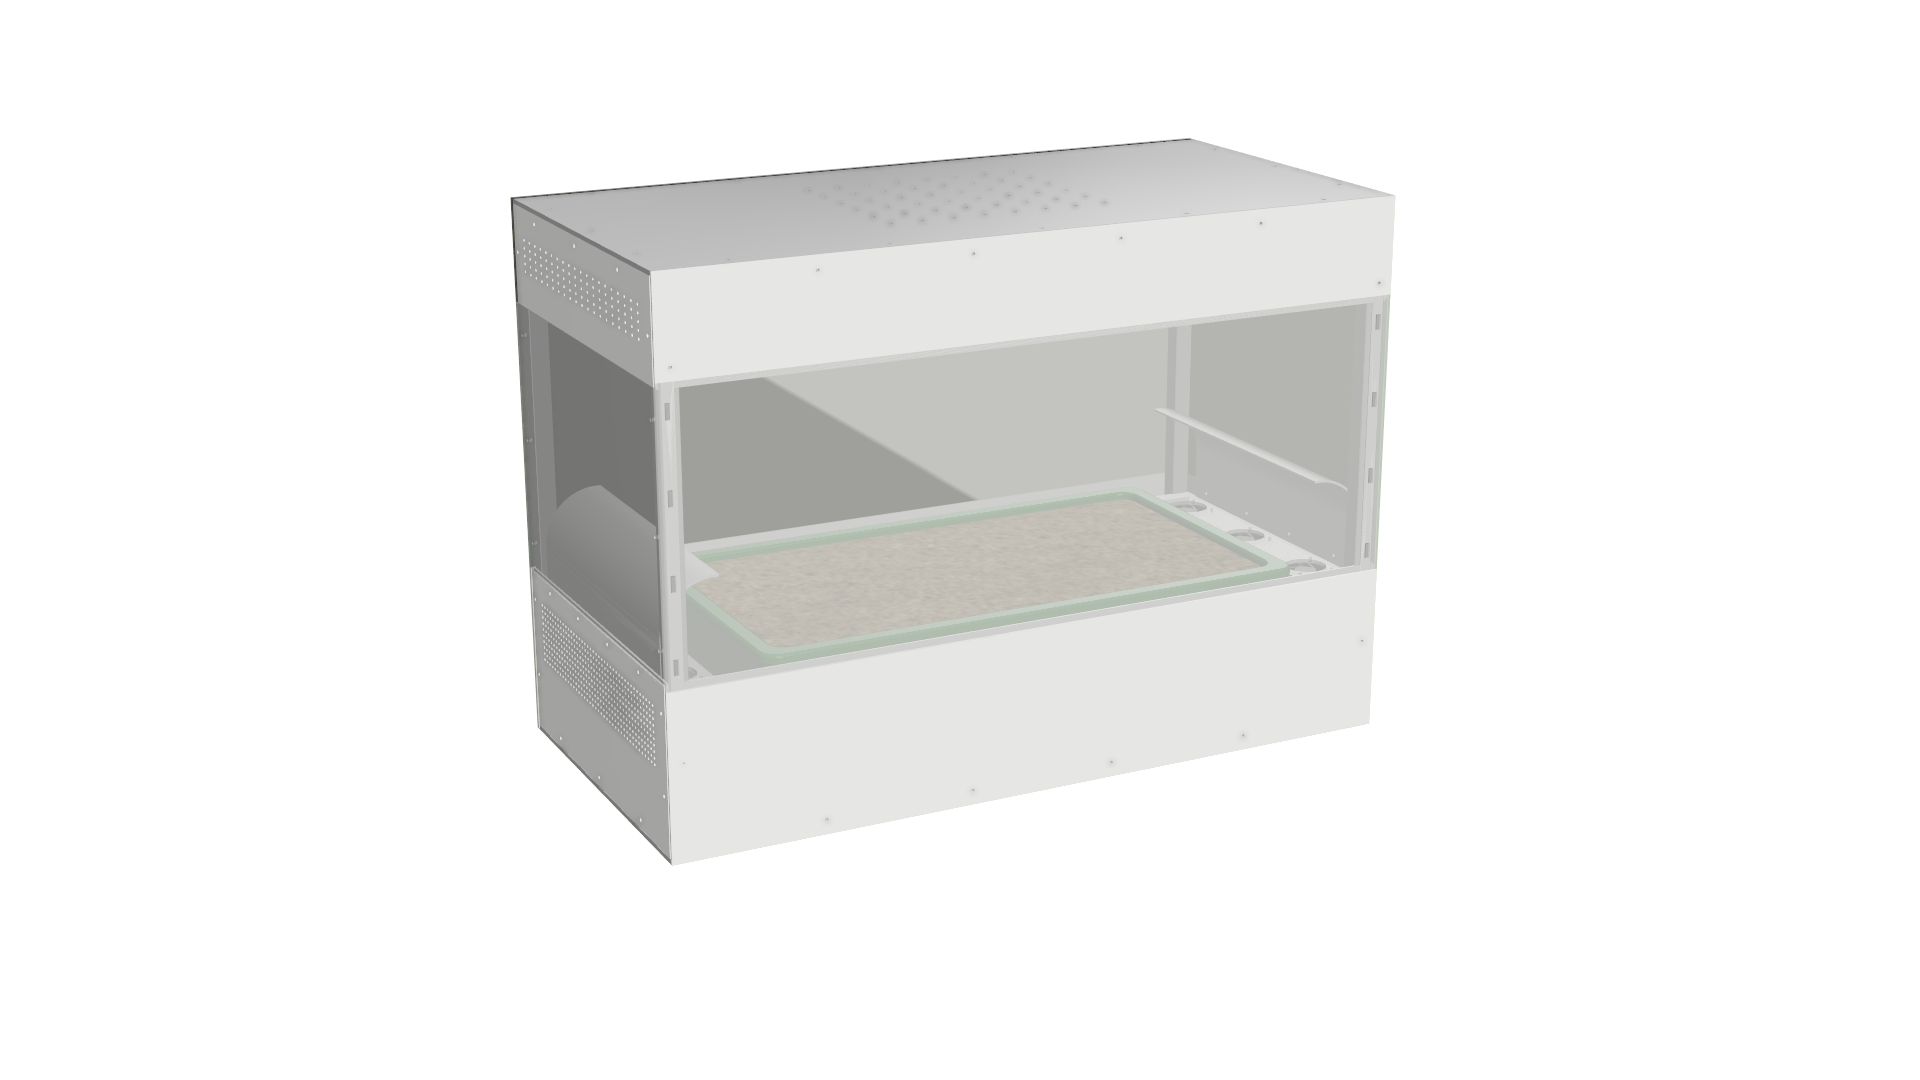
\includegraphics[width=400pt]{version2}\\
To see the 3D Model  \href{http://a360.co/2sLIiCD}{Click}\\
\href{https://www.youtube.com/watch?v=ab_HcFKEwkE}{Air Flow Simulation in Grow Box Version2} in Solid Works\\
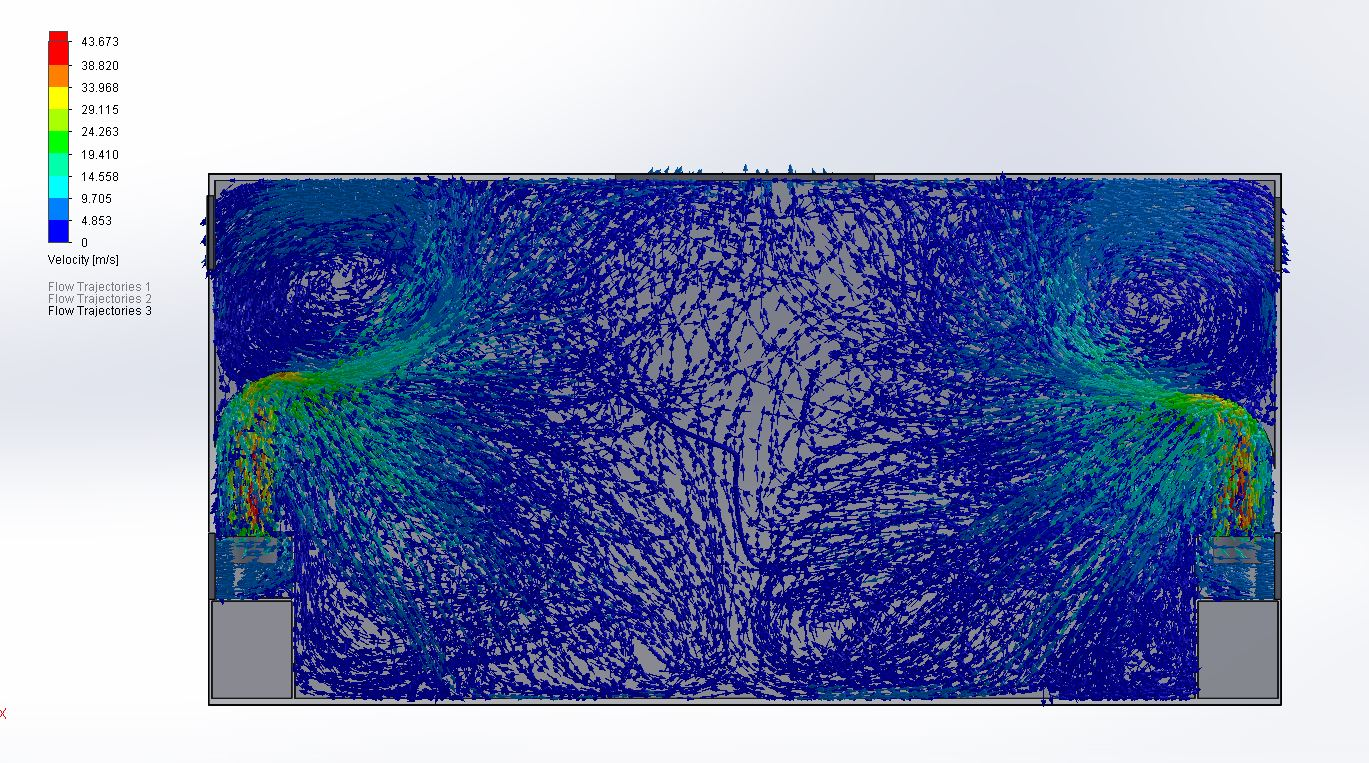
\includegraphics[width=200pt]{version_2_FV}
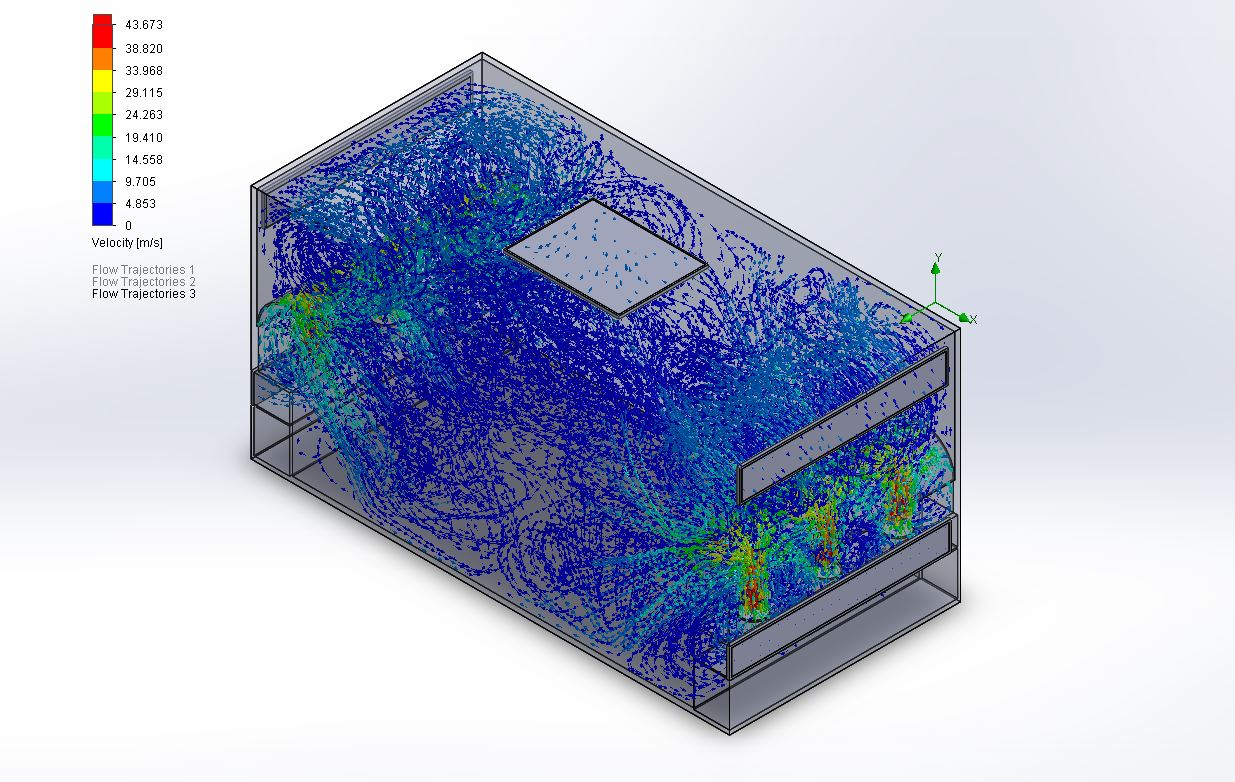
\includegraphics[width=200pt]{version_2_ISO}
Reasons why this model has been fabricated-
\begin{itemize}
    \item Good air flow inside the Grow Box.
    \item Less cost compared to version1 design.
    \item DIY design, as design is not complex, so anyone can assemble it with ease.
    \item This design is modular. So, it can be stacked vertically or horizontally by just changing the Aluminum Tube with MS Tubes.
    \item This design is smaller in size compared to existing and version1 model.
\end{itemize}
The disadvantage of this model are- 
\begin{itemize}
\item There is no provision of water storage. So water level have to be checked regularly. 
\item This design have no provision for exhaust fans. In this design number of inlet fans have been increased to compensate for exhaust fans.
\end{itemize}

\section{Hardware parts}
\begin{itemize}
  \item List of hardware
  \begin{enumerate}
  \item Square Aluminum Pipe
  \item Square Connectors
  \item Clear Acrylic Sheets
  \item Opaque Acrylic Sheets
  \item Fasteners
  \item Magnets
  \item Aluminum or Mild Steel Strips
  \item Axial Flow Fans
  \item SunBoard or Foam Board
  \item Brackets
  \end{enumerate}
  \item Detail of each hardware:\\\\
  Different parts of Grow Box are as follows:
   \begin{enumerate}
  \item Square Aluminum Pipe  \href{https://www.justdial.com/Mumbai/Variety-Aluminium-Ghatkopar-West/022P1932129_BZDET}{Vendor link},\\
  Aluminum Square tubing is used as supporting structure because of its light weight, relative strength, superior resistance to corrosion and easy to work with properties.\\
  When vertical stacking is needed these Aluminum tubing can be replaced by High strength steel pipes due to more relative strength.
  \begin{enumerate}
  \item \href{http://a360.co/2sqg5SJ}{Tube 93.2}
  \item \href{http://a360.co/2tpFQUh}{Tube 43}   
  \item \href{http://a360.co/2tpFQUh}{Tube 65}   
  \end{enumerate}
  \item Square Connectors\href{https://www.indiamart.com/digitalmetrology/tube-connector.html}{Vendor link},\\
  No fasteners are required to fix them, friction holds the framing together. This makes it easy to use and anyone can join these like Lego blocks.
  \begin{enumerate}
  \item \href{http://a360.co/2sMp2oQ}{3 Way 90deg Elbow Square Connectors} 
  \end{enumerate}
  \item Clear Acrylic Sheets\\
  These provide clear view of the plants inside. These are mainly provided for aesthetic look. These also acts as supporting structures.\\
  Front mid panel is attached to the framing structure using magnets. This can be removed when needed.
  \begin{enumerate}
  \item \href{http://a360.co/2sq8qUr}{Front Mid Panel}
  \item \href{http://a360.co/2sGPxAG}{Rear Mid Panel}   
  \item \href{http://a360.co/2thgj1m}{Right Side Mid Panel} 
  \item \href{http://a360.co/2thgj1m}{Left Side Mid Panel}
   \item \href{http://a360.co/2tJ37U7}{Side Curve Panel}
  \end{enumerate}
  \item Opaque Acrylic Sheets\\
  These are used to hold the outer aluminum structure together and thus acting as supporting structures.These are attached to the aluminum tubes using screws. These are opaque to hide the turf, electronics and lights.
  \begin{enumerate}
  \item \href{http://a360.co/2sGEDLo}{Front Top Panel}
  \item \href{http://a360.co/2sqkqoI}{Front Bottom Panel}
  \item \href{http://a360.co/2th6yjx}{Rear Top Panel} 
  \item \href{http://a360.co/2thjbLA}{Rear Bottom Panel}
  \item \href{http://a360.co/2sGqayR}{Right Side Top Panel}  
  \item \href{http://a360.co/2sGInMZ}{Right Side Bottom Panel}
  \item \href{http://a360.co/2sGqayR}{Left Side Top Panel}
  \item \href{http://a360.co/2sGInMZ}{Left Side Bottom Panel}
  \item \href{http://a360.co/2tJ6avt}{Top Panel}
  \item \href{http://a360.co/2tIuY6K}{Base Panel}
  \item \href Component Box Panels
  \begin{enumerate}
  \item \href{http://a360.co/2sGOZLh}{Top Panel}
  \item \href{http://a360.co/2tpwkkd}{Side Panel}
  \item \href{http://a360.co/2sMPwGt}{Rear Panel}
  \item \href{http://a360.co/2sGHmog}{Partition Panel}
  \end{enumerate}
   \end{enumerate}
  \item Fasteners\\
  Fasteners are used to attach acrylic sheets to aluminum tubes together. 
  \begin{enumerate}
  \item Screw\\
  Diameter of the screw used here is 1/8 inches.
  \item Screw Bolts
  \item Screw Nuts
  \item Butterfly Nut
  \item Bolt
  \end{enumerate}
  \item Magnets\href{http://www.amazon.in/Perfect-Magnets-Nickel-Coated-Pieces/dp/B01LY18VN3/ref=sr_1_7?ie=UTF8&qid=1499193943&sr=8-7&keywords=magnets}{ Vendor link},\\
  These are used to hold the front mid panel. Using these removes latches to hold the panel, thus removing any protrusions. 
  \item Mild Steel/Aluminum Strips\\
  These are used to hold the LED Flood Lights.
  \begin{enumerate}
  \item \href{http://a360.co/2sGs5DH}{Light Holders}
   \end{enumerate}
  \item Sun Board or Foam Board\\
   Sunboard acts as sealing agent by not allowing the air inside to leak from sides
  \item Brackets
  \item Axial Flow Fans\href{http://www.amazon.in/60x60x25mm-Brushless-12V-Cooling-Fan/dp/B01MS9AHPC/ref=sr_1_99?ie=UTF8&qid=1499194646&sr=8-99&keywords=dc+fans+12v}{ Vendor link},\\
  An axial fan is a type of a compressor that increases the pressure of the air flowing through it. The blades of the axial flow fans force air to move parallel to the shaft about which the blades rotate.\\
  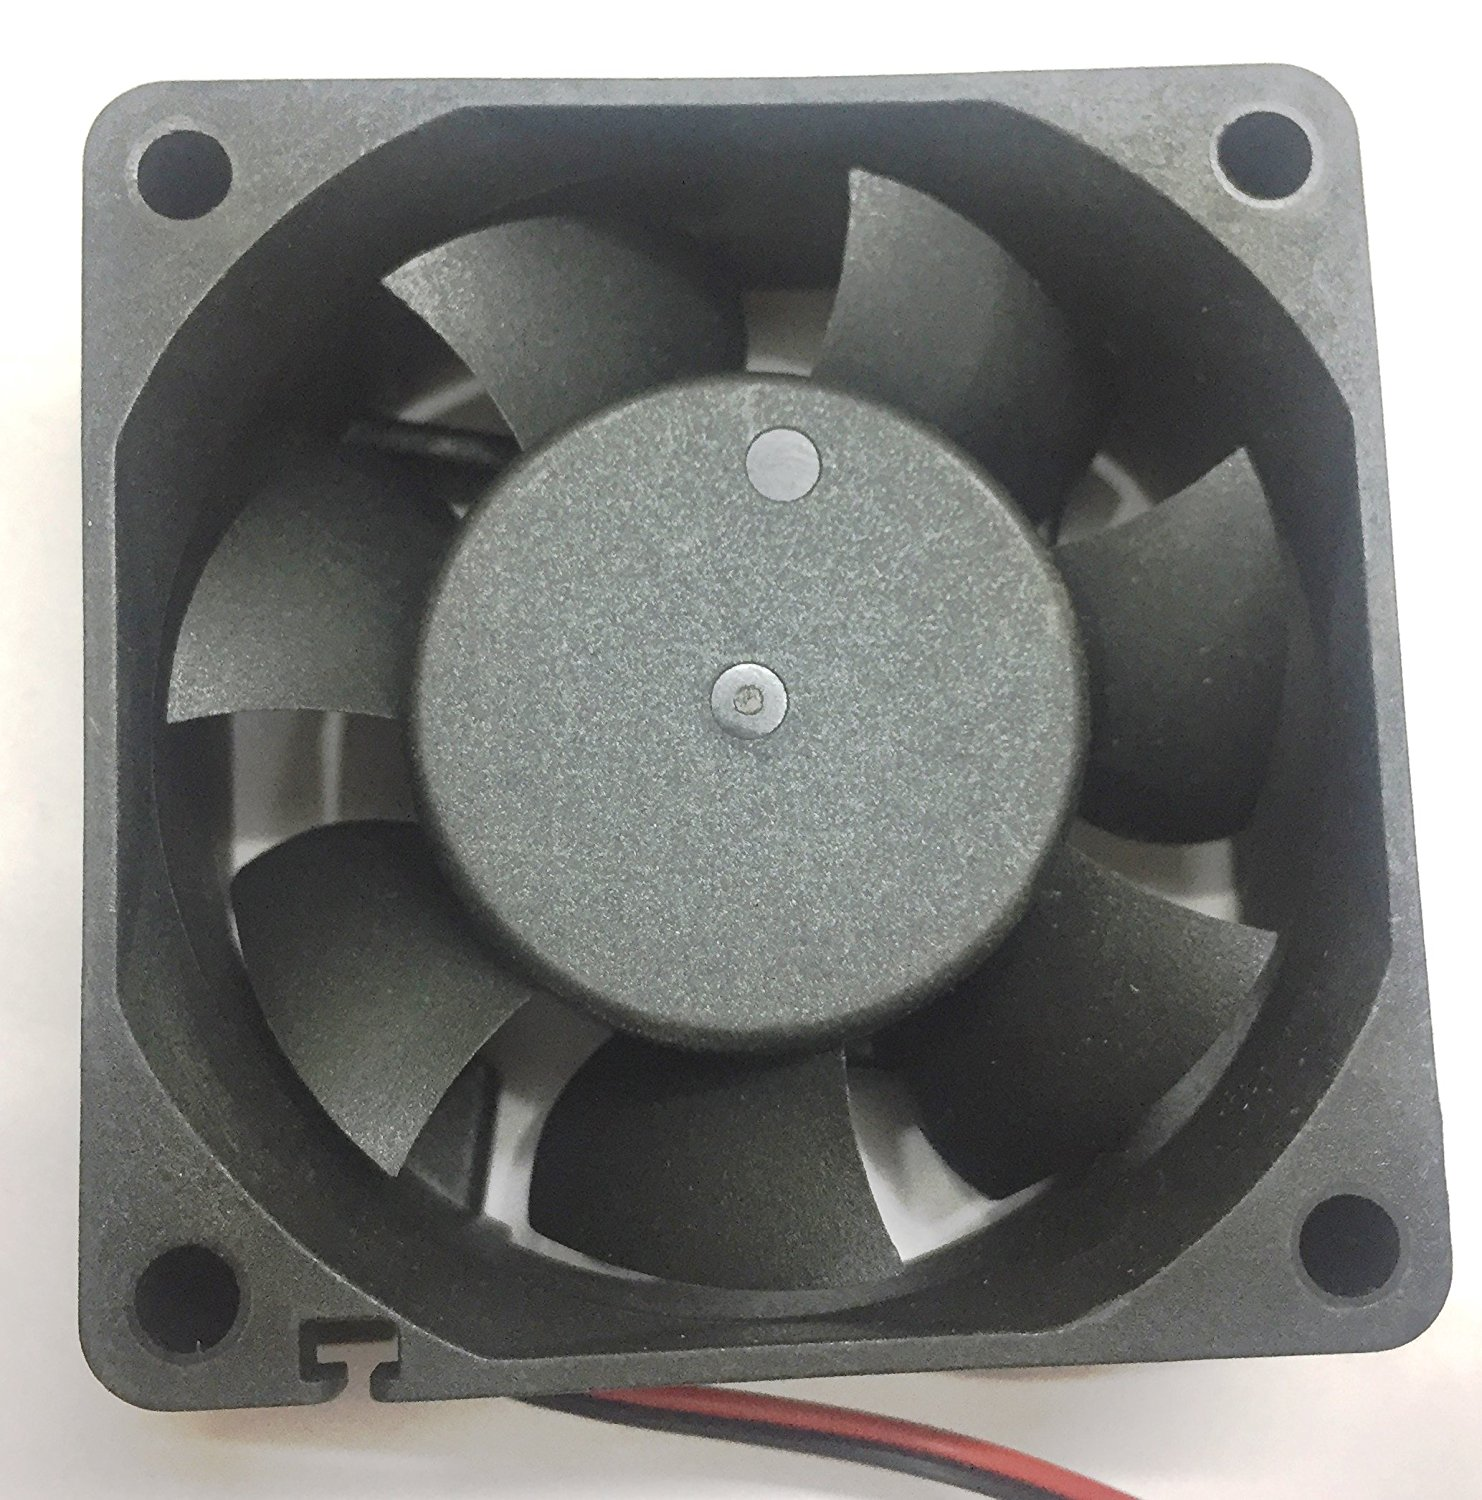
\includegraphics[width=200pt]{Fan60x60x25}\\
  Product specification voltage: 12v current: 0. 12 - 0. 21 a dimensions: 60 x 60 x 25 mm (lxwxh) DC brushless motor fan brand can be different as shown in picture but other features and dimensions will remain same. Application: Cnc, robotics, DIY projects, computer cases, power supplies, 12v circuits where cooling is required. Package include: 1 x 60x60x25mm cooling fan.
  \end{enumerate}
\end{itemize}


\section{Assembly of hardware}
Steps of assembly of hardware with pictures for each step.
\subsection*{Steps to Assembly}
\subsection*{Step 1}
Press fit the 3 way joint to aluminum tube and hammer with a rubber mallet.\\
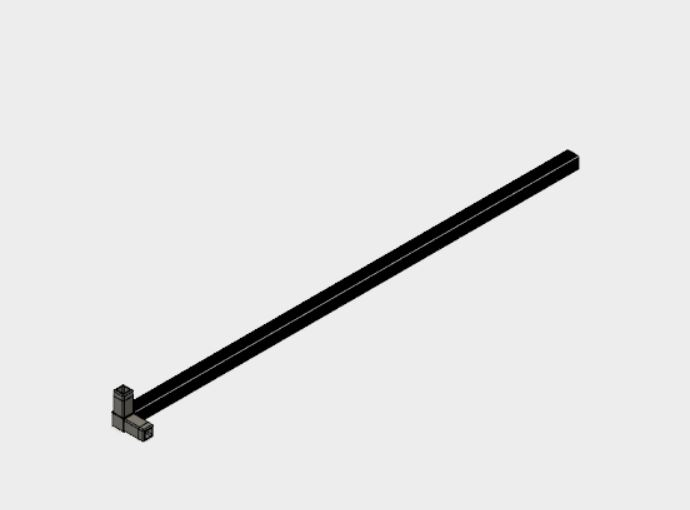
\includegraphics[width=200pt]{1}
\subsection*{Step 2}
Similarly press fit the other 3 way joint to aluminum tube and hammer with a rubber mallet.\\
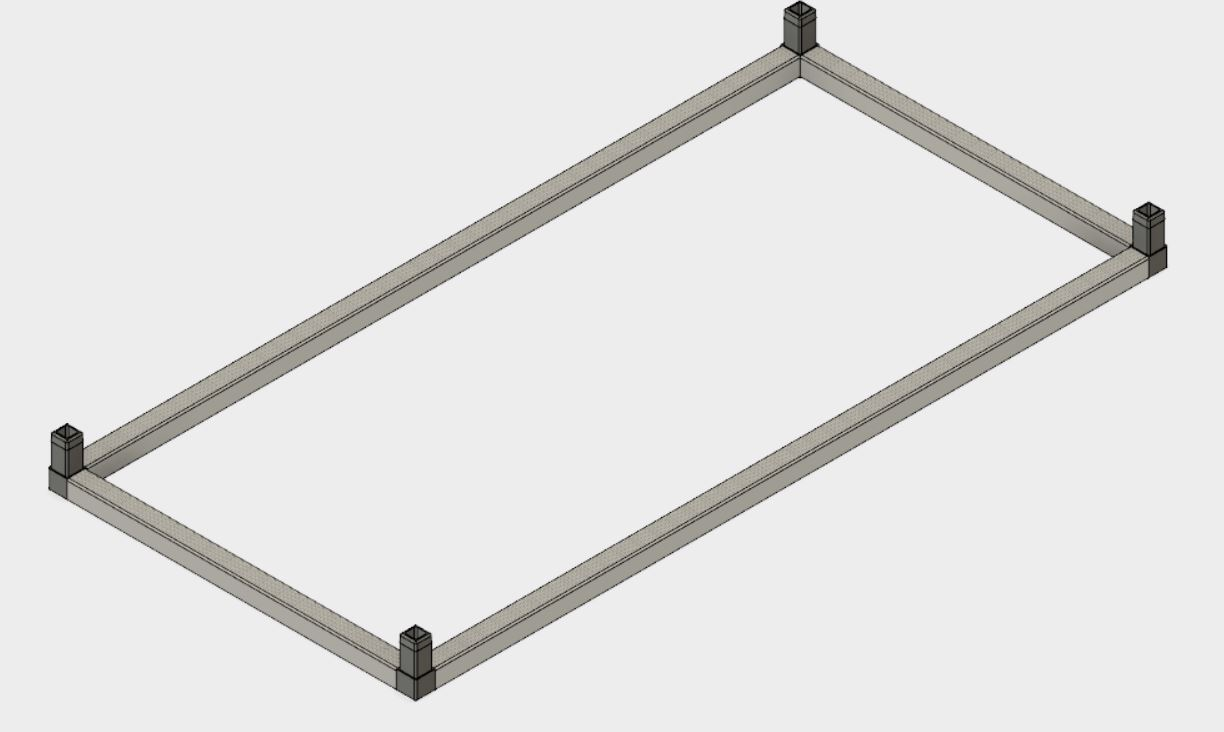
\includegraphics[width=200pt]{2}
\subsection*{Step 3}
Fix the base panel to the frame using screws.\\
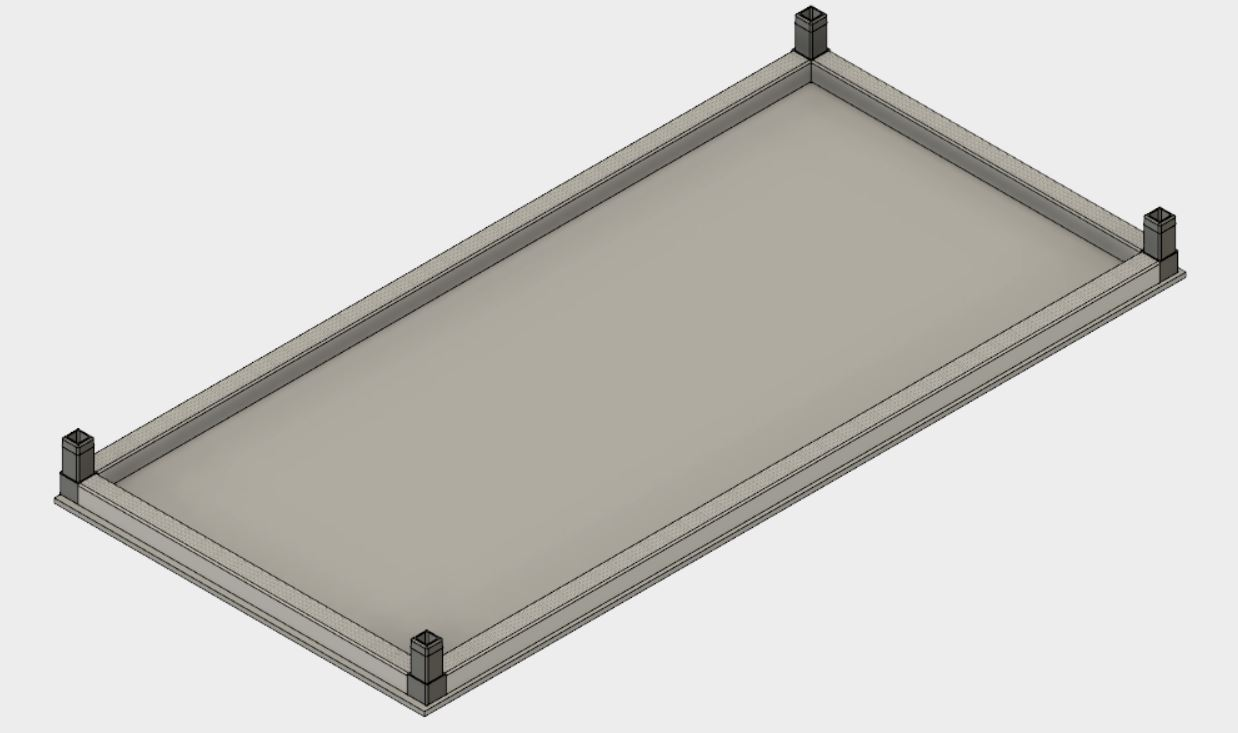
\includegraphics[width=200pt]{3}
\subsection*{Step 4}
Press fit the vertical aluminum tubes to the 3 way connectors and hammer with a rubber mallet.\\
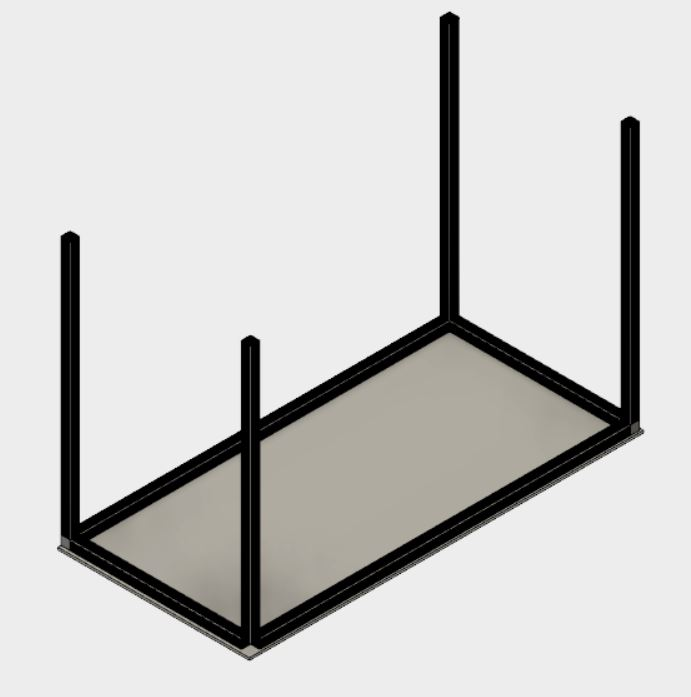
\includegraphics[width=200pt]{4}
\subsection*{Step 5}
Similarly press fit the top frame with 3 way joint to aluminum tube and hammer with a rubber mallet.\\
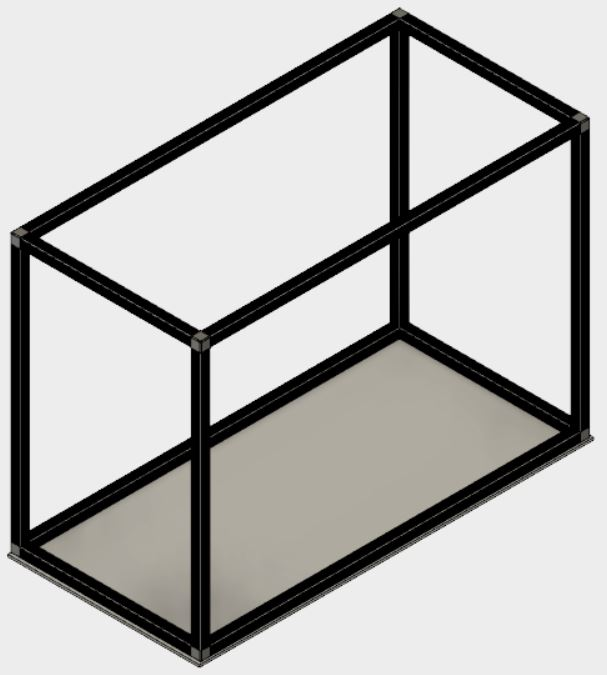
\includegraphics[width=200pt]{5}
\subsection*{Step 6}
Fix the bottom panels of front, rear and sides to the frame using screws.\\
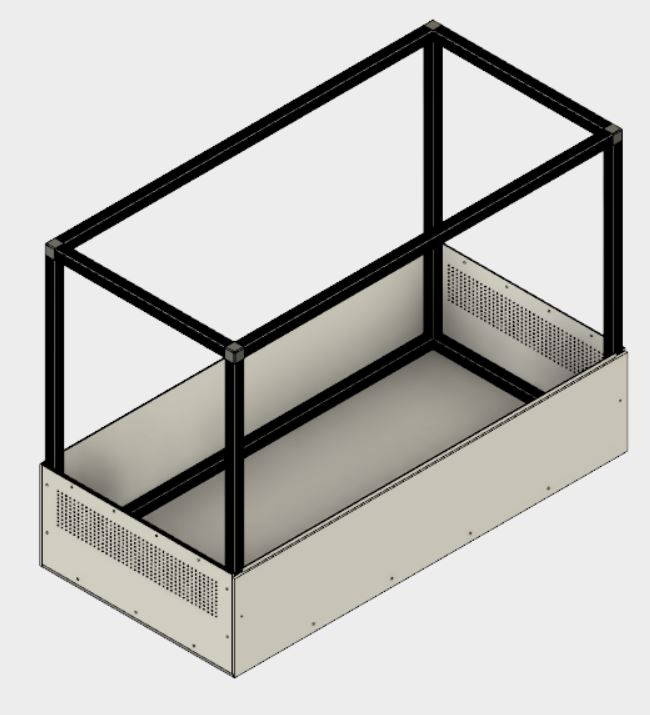
\includegraphics[width=200pt]{6}
\subsection*{Step 7}
Attach the mid panels of rear and sides to the frame using screws.\\
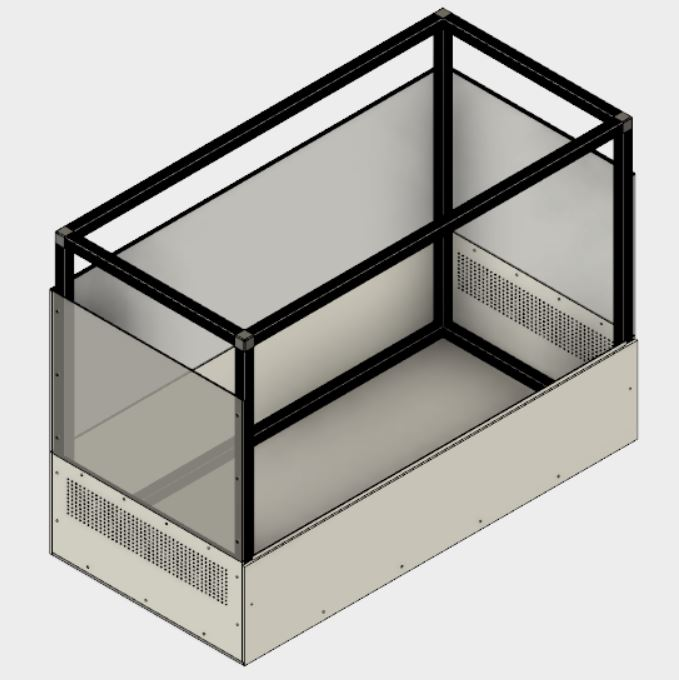
\includegraphics[width=200pt]{7}
\subsection*{Step 8}
Similarly attach the top panels of front, rear and sides to the frame using screws.\\
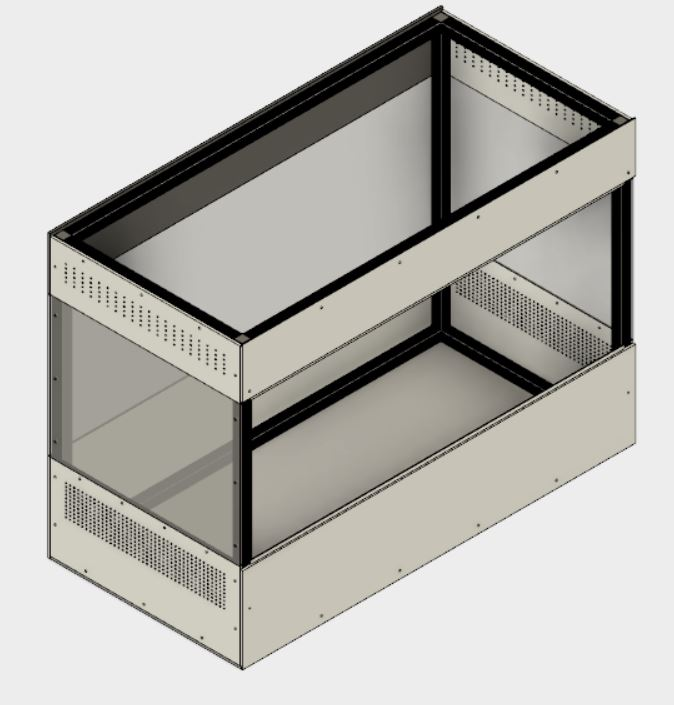
\includegraphics[width=200pt]{8}
\subsection*{Step 9}
Attach the top panel to the frame using screws.\\
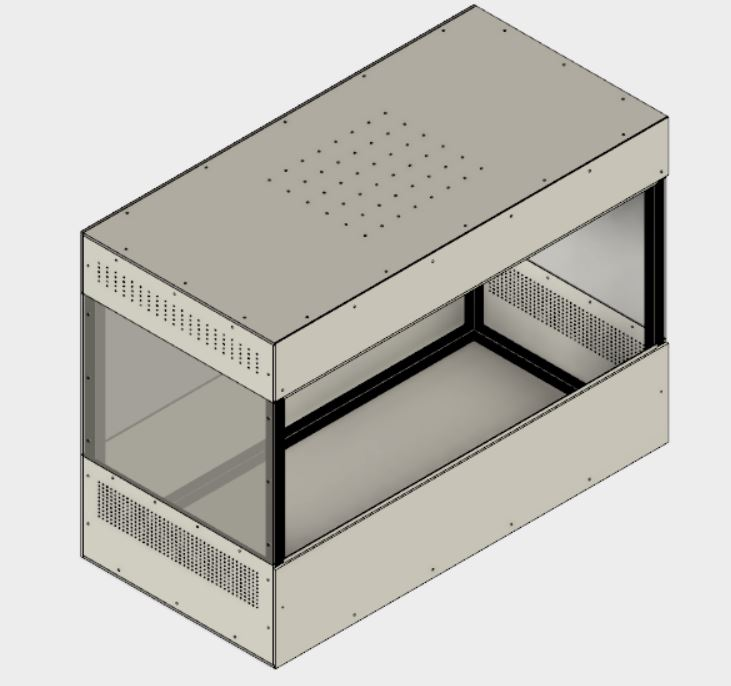
\includegraphics[width=200pt]{9}
\subsection*{Step 10}
Assemble the component box as shown in figure using chloroform.\\
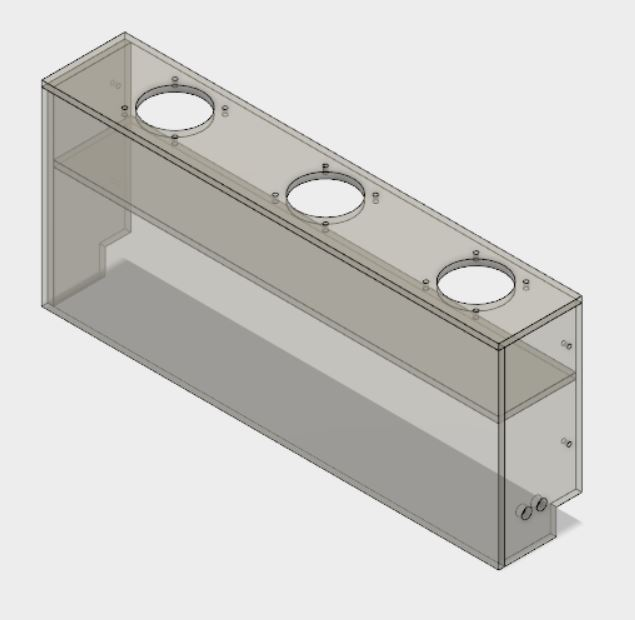
\includegraphics[width=200pt]{10}
\subsection*{Step 11}
Fix the fans to the component box using screws and nuts.\\
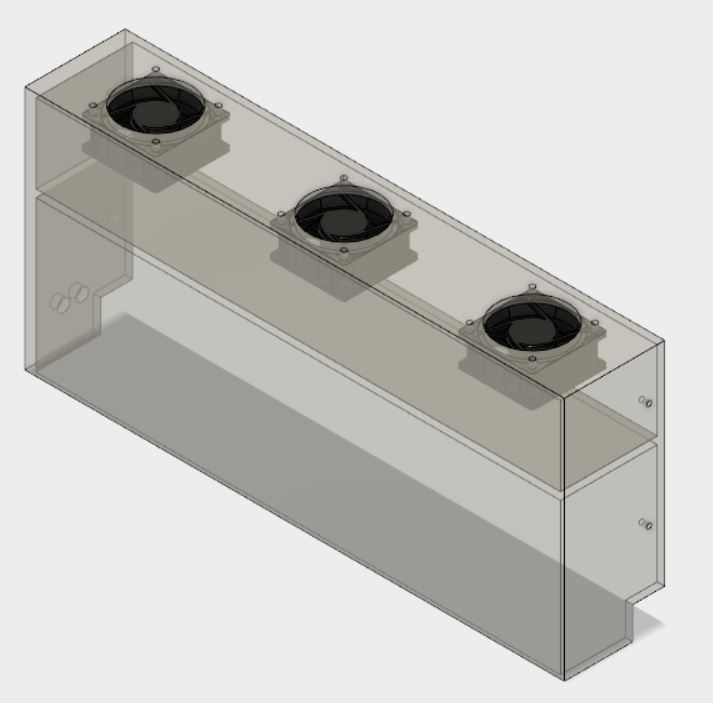
\includegraphics[width=200pt]{11}
\subsection*{Step 12}
Place the component box inside the box as shown in figure and fix them with the help of L brackets and screws.\\
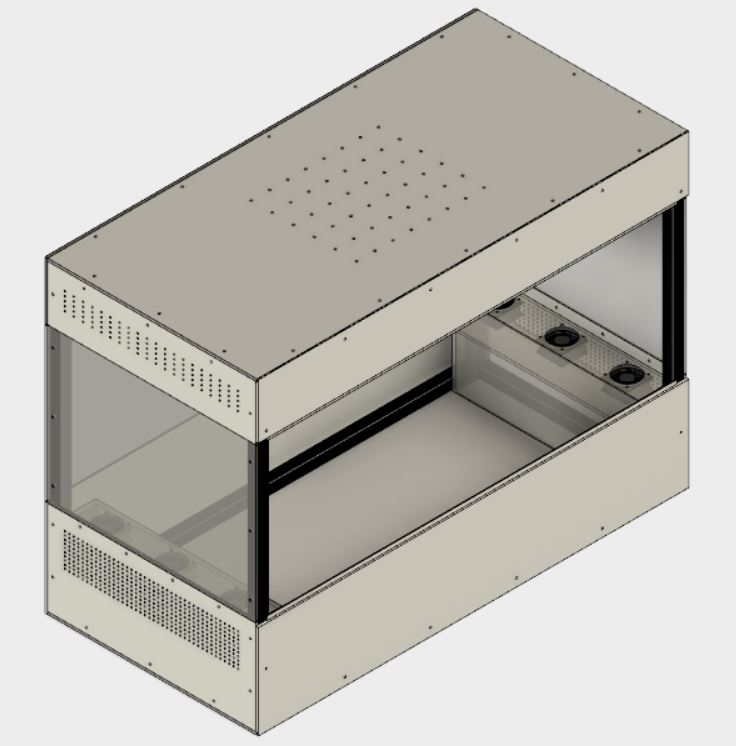
\includegraphics[width=200pt]{12}
\subsection*{Step 13}
Remove the bottom panels of sides and assemble the Electronic components inside the box. \\
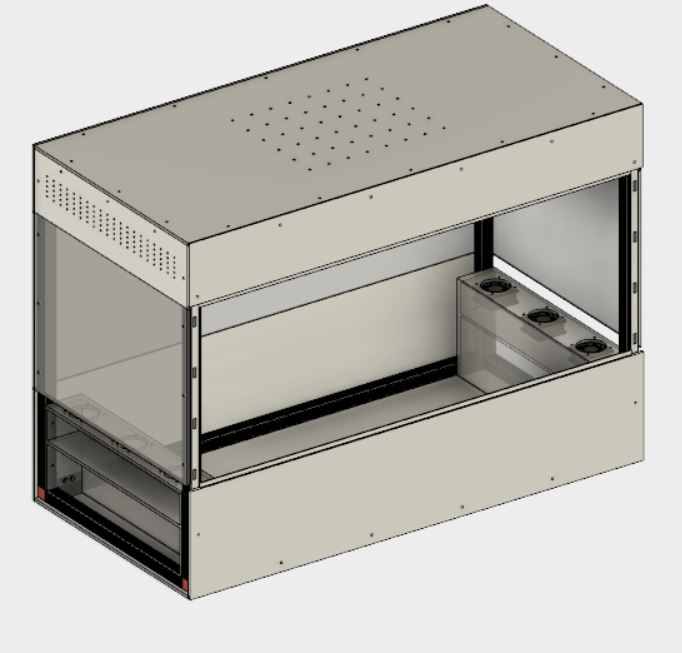
\includegraphics[width=200pt]{13}
\subsection*{Step 14}
Attach the bottom panels of sides and the curve panel using screws.\\
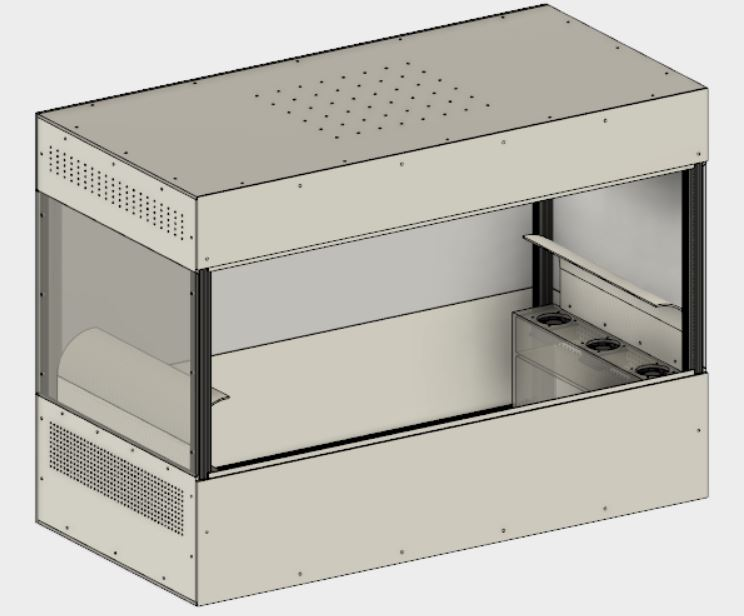
\includegraphics[width=200pt]{14}
\subsection*{Step 15}
Fix the light holding Aluminum or Mild Iron Strip to the top frame using screws .\\
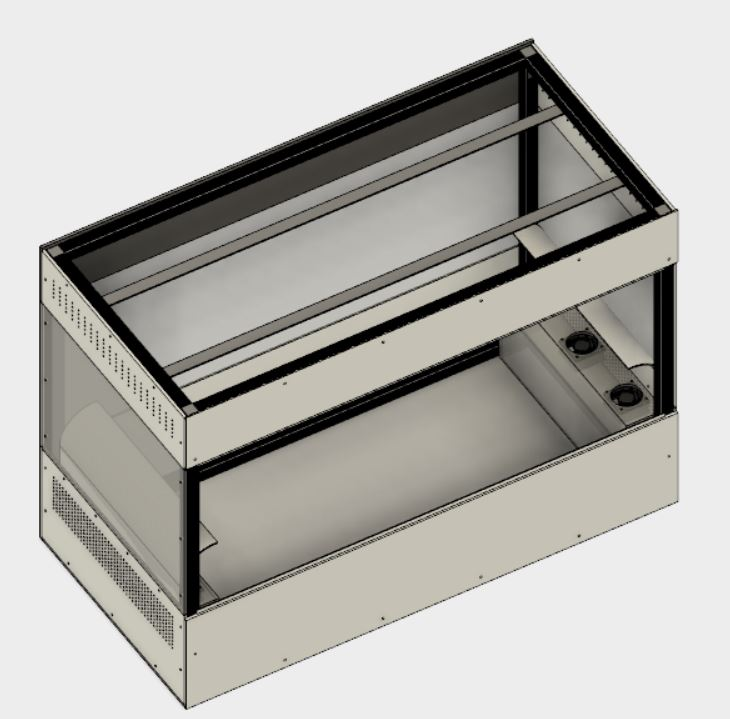
\includegraphics[width=200pt]{15}
\subsection*{Step 16}
Fix the sunboard or foam board and magnets on the front side of frame as shown in figure with the help of Fevi Quick and let it cure for some time. Put masking tape above the sunboard and magnets.\\
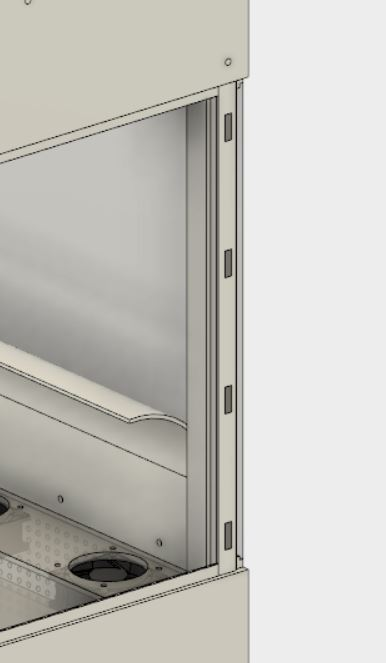
\includegraphics[width=200pt]{16}
\subsection*{Step 17}
Fix the magnets in the grooves provided in front mid panel using Fevi Quick or Araldite and let it cure for sometime. Put masking tape on the magnets. Take care of polarity of the magnets. Now front mid panel can be attached and removed as required.\\
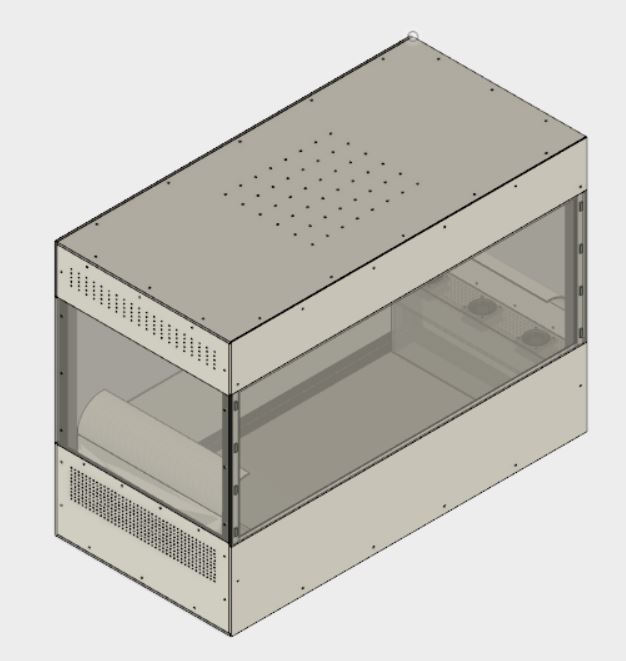
\includegraphics[width=200pt]{17}
\subsection*{Step 18}
Remove the front mid and bottom panels to pace the Turf inside the Grow Box. Attach the panels back to the frame.\\
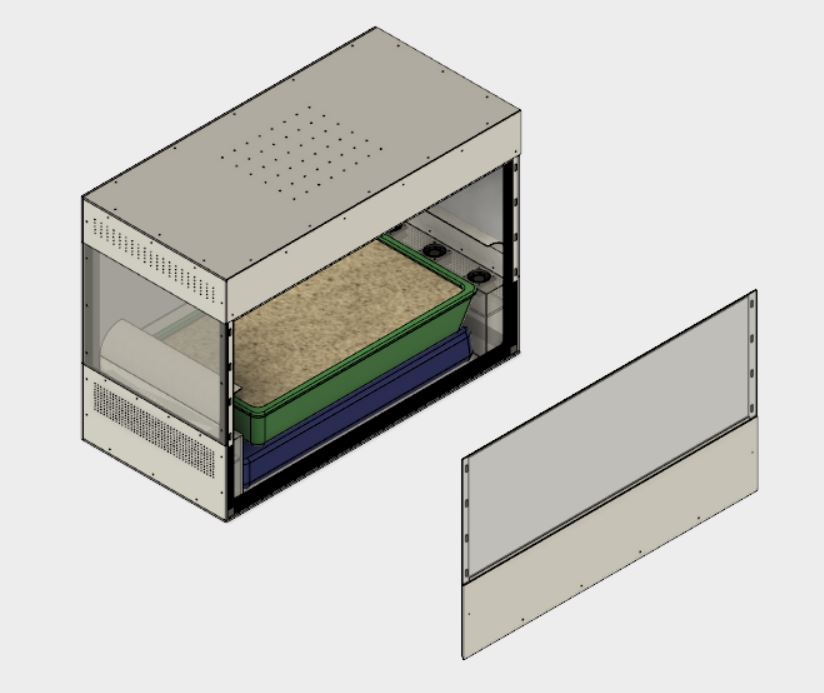
\includegraphics[width=200pt]{18}



\section{Future Work}
\begin{itemize}
\item Top panel needs to be redesigned in order to allow cooling of LED Flood Light.
\item To control temperature, Heater and chiller unit need to be added.
\item To control humidity, Humidifier need to be added.
\item Carbon filters need to be added at exhaust end to remove any smell from plants.
\end{itemize}

\section {Design Files}
\subsection{CAD Model Files}
\begin{itemize}
    \item \href{https://drive.google.com/file/d/0B8nJz0e_p6YNYkN4LWZJdHdqNEE/view?usp=sharing}{Version1 Models}
    \item \href{https://drive.google.com/open?id=0B8nJz0e_p6YNaC00T0h0N1Y0VVE}{Version2 Models}
\end{itemize}
\subsection{Flow Simulation Files}
\begin{itemize}
    \item \href{https://drive.google.com/open?id=0B8nJz0e_p6YNY2tDaUpiR3BRZXc}{Version0}
    \item \href{https://drive.google.com/open?id=0B8nJz0e_p6YNaVZpd2Y5OVdYSVE}{Version1}
    \item \href{https://drive.google.com/open?id=0B8nJz0e_p6YNTGNyNHEzUktRTFk}{Version2}
\end{itemize}

\begin{thebibliography}{li}
\bibitem{wavelan97}
Ad Kamerman and Leo Monteban,
{\em WaveLAN-II: A High-Performance Wireless LAN for the Unlicensed band},
1997.

\end{thebibliography}


\end{document}

